\begin{abstract}
Climate change and various anthropogenic factors significantly influence biodiversity and population evolutionary dynamics. To deepen our understanding of the mechanisms driving these disturbances within ecosystems, biologists employ phylogeographic approaches. These methods aim to establish the correlation between the genetic structure of populations and their geographical distribution, considering their current or historical geoclimatic history.

We focus on developing bioinformatics  \textbf{aPhyloGeo} tools to enhance phylogeographic analysis. Recognizing the urgency of the current climate crisis, we are conducting an in-depth analysis of the impact of extreme climatic parameters and environmental factors on Cumacea (crustaceans: Peracarida). Our approach includes a comparative study that validates our phylogeographic models against environmental data from the northern waters of the North Atlantic around Iceland. Concurrently, we are updating a Python package (\url{https://github.com/tahiri-lab/aPhyloGeo}), also available on \href{https://pypi.org/project/aphylogeo/}{PyPi}, to facilitate these complex analyses.
\end{abstract}

\section{Introduction}\label{introduction}
In the expansive North Atlantic and subarctic region, the Icelandic area and its adjacent waters offer compelling ecological intrigue \citep{schnurr_composition_2014, uhlir_adding_2021}. These waters harbor a diverse array of water bodies from various origins, often interacting and overlapping \citep{uhlir_adding_2021}. Characterized by specific oceanographic and hydrographic features, these waters shape benthic habitats through depth gradients, water mass indicators, and habitat arrangements \citep{uhlir_adding_2021}. Consequently, research conducted in these regions enhances our comprehension of deep-sea ecosystems and the associated biodiversity patterns within them \citep{meisner_prefacebiodiversity_2018, uhlir_adding_2021}.

The biological and environmental baseline data gathered in these regions by projects like IceAGE, as well as its predecessors BIOFAR and BIOICE, are invaluable resources \citep{meisner_prefacebiodiversity_2018}. These projects focused on studying biodiversity in the Faroe Islands and Iceland \citep{meisner_prefacebiodiversity_2018}. Such data provide crucial insights into understanding two significant challenges facing current and future generations: the impacts of climate change and seabed mining. The North Atlantic region surrounding Iceland has long been recognized as pivotal for global thermohaline circulation regulation \citep{meisner_prefacebiodiversity_2018}. The Greenland, Iceland, and Norwegian (GIN) seas, alongside the high-latitude North Atlantic, play vital roles in modern deep-sea ventilation and global thermohaline circulation \citep{johannessen_relationship_1994}. Notably, significant changes, such as the formation of cold, deep water, have been observed \citep{meisner_prefacebiodiversity_2018}. The loss of Arctic sea ice has slowed down the deep-sea formation process, potentially impacting flow dynamics and chemistry, as observed during the IceAGE expedition \citep{meisner_prefacebiodiversity_2018}.

There is a burgeoning international interest in deep-sea resource extraction, with mining operations set to commence in some areas \citep{mengerink_call_2014}. These operations primarily target mid-ocean ridges and other active geothermal sites, including those around Iceland, such as the Reykjanes Ridge, known for its hydrothermal vent sites. Accurately assessing the extent of damage and loss of ecosystem services due to mining activities necessitates robust baseline data \citep{meisner_prefacebiodiversity_2018}.

Crustaceans belonging to the taxon Peracarida Calman, 1904, often comprise a significant proportion of macrobenthic communities in Arctic and subarctic waters \citep{uhlir_adding_2021}. They are widely dispersed across the continental shelf and slope of northern seas \citep{uhlir_adding_2021}. This study focuses on the peracarid taxon Cumacea Krøyer, 1846, predominantly bottom-dwelling marine benthic crustaceans that spend a substantial part of their lives buried in or near sediments \citep{uhlir_adding_2021}. Consequently, Cumacea are presumed to have limited dispersal abilities and are unlikely to move great distances \citep{uhlir_adding_2021}.

In contrast to benthic invertebrates inhabiting rocky intertidal environments in the Northwest and Northeast Atlantic, information regarding the evolutionary history and dynamics of deep-sea benthic invertebrates in the North Atlantic remains limited \citep{jennings_phylogeographic_2014}. While studies have revealed intriguing genetic distribution patterns of deep-sea benthic invertebrates, such as a homogenous genetic structure with the expansion of North Atlantic populations towards the poles, it is imperative to deepen our understanding of the origin and demography of deep Atlantic biota. This understanding is essential for elucidating their contemporary connectivity in an evolutionary context and their relationship with ongoing climate change. Continued warming may lead to the opening up of transarctic routes \citep{jennings_phylogeographic_2014}.

Against the backdrop of the current climate emergency, this study aims to conduct an in-depth analysis of the influence of extreme climatic parameters and environmental peculiarities on Cumacea (crustaceans: Peracarida). Specifically, we aim to ascertain whether there is a correlation between the genetic information of regions of the mitochondrial 16S rRNA gene of these species and the physical characteristics of their habitats. Our approach includes a comparative study to validate different phylogeographic models by comparing them with environmental factors found in the waters of the North Atlantic around Iceland. Additionally, we will update a Python package (in beta) to facilitate these complex analyses.

\section{Related Works}\label{related-works}
Many studies have investigated the relationship between genetics and the climatic conditions of their study region. These studies have provided a better understanding of how organisms adapt to their habitat and evolve in it over time \citep{fc_genomic_2012}. They have also helped develop conservation plans to maintain biodiversity and protect endangered species by designing how populations are adapted to their environment.

\cite{koshkarov_phylogeography_2022} proposed a phylogeographic approach based on an algorithm called aPhyloGeo to study the correlation between Severe acute respiratory syndrome coronavirus 2 (SARS-CoV-2) variants and their geographical characteristics. More recently, \cite{li_aphylogeo-covid_2023} have developed an interactive platform called aPhyloGeo-Covid to facilitate these analyses.  We elaborate on the aPhyloGeo software as well as its use in this study later in this article.

A study by \cite{ghalambor_adaptive_2007} has demonstrated that habitat characteristics, such as water temperature, can affect the genetics of guppy populations (Poecilla reticulata) by shaping their phenotypic plasticity as well as by promoting rapid genetic adaptation. \cite{cheviron_genomic_2012} also concluded that there was a correlation between vertebrate genetics and habitat properties, particularly in extreme environments such as high altitudes. This correlation between genetics and environmental characteristics was also supported by the results of studies of Threespine Sticklebacks \citep{fc_genomic_2012}. Those results aren't surprising consider that species acclimatization to climate change is often the result of the interaction between genetic variation among populations and selection pressures caused by environmental changes.

However, studies have highlighted the complexity of the relationships between genetics and the environment that can be influenced by many factors such as genotype-environment interaction and natural selection. This can make it difficult to identify unambiguous causal relationships between these two parameters \citep{manel_perspectives_2010}. Other studies mention that it is difficult to distinguish between the direct and indirect effects of the environment on genetics \citep{manel_perspectives_2010, balkenhol_landscape_2019}. Studies of the effect of the environment on the genetics of organisms may be limited by the methods available to measure genetic and environmental characteristics, as well as by logistical constraints related to data collection and generation \citep{manel_perspectives_2010, shafer_widespread_2013}. To our knowledge, this last point must contribute in particular to the fact that research on the environment and genetics of Cumacea is little explored.

As stipulated in hypothesis of Darwin, individuals best adapted to their environment are likely to survive, reproduce and evolve. The objective of this study is to deepen and strengthen the natural selection hypothesis by examining whether there are one or more locations within Cumacea DNA sequences that could better correlate them with their environment.


\section{Materials and Methods}\label{materials-methods}

\subsection{Description of the data}
The study area is located in a northern area of the North Atlantic, including the Icelandic Sea, the Denmark Strait, and the Norwegian Sea. The specimens included in this study were collected during the international IceAGE (Icelandic marine Animals: Genetic and Ecology; Cruise ship M85/3 in 2011; \citep{meisner_prefacebiodiversity_2018}) aboard the Meteor RV that explored the deep continental slopes and abyssal waters around Iceland \citep{meisner_prefacebiodiversity_2018}. The data considered in this study from the IceAGE expedition are available via the study of \cite{uhlir_adding_2021}. The sampling period for the specimens included in this study is from August 30 to September 22, 2011, and they were collected in a depth range of 316-2568 m. A description of the sampling plan and sample processing is provided in \cite{uhlir_adding_2021}. The steps of DNA extraction, PCR amplification and sequencing, as well as the extracted and aligned DNA sequences, are also available in the article by \cite{uhlir_adding_2021}.

\subsection{Data pre-processing}
We considered data from the IceAGE project as well as data from the BOLD Systems database, both of which are available via the article by \cite{uhlir_adding_2021}. Given the large range of attributes from these databases, we made a succinct selection of the number of attributes and samples across them. Thus, we omitted attributes that were not relevant in the context of this study, that were completely or nearly invariable (non-numerical data) as well as those that had abundant missing data (> 95\%). We considered 62 of the 495 datasets from the IceAGE project.

Subsequently, we calculated the variance for each of the selected numeric attributes in order to eliminate those with zero or low variance (cut-off ≥ 0.1):

\begin{equation}
S^2 = \frac{\sum_{i=1}^{n} (x_i - \bar{x})^2}{n-1}
\end{equation}

where \( S^2 \) is the variance of the sample, \( x_i \) represents each value in the data set, \( \bar{x} \) the average of all values in the data set, and \( n \) the number of values in the data set.

Of the previously selected numerical attributes, only salinity was removed (\( S^2 = 0.02146629 \)). This selection of attributes and data resulted in a data table containing 62 rows (\( n=62 \)) and 18 columns (number of attributes). Figures \ref{fig:fig1} and \ref{fig:fig2} were made from Python 3.11.

\begin{figure}[]
    \centering
    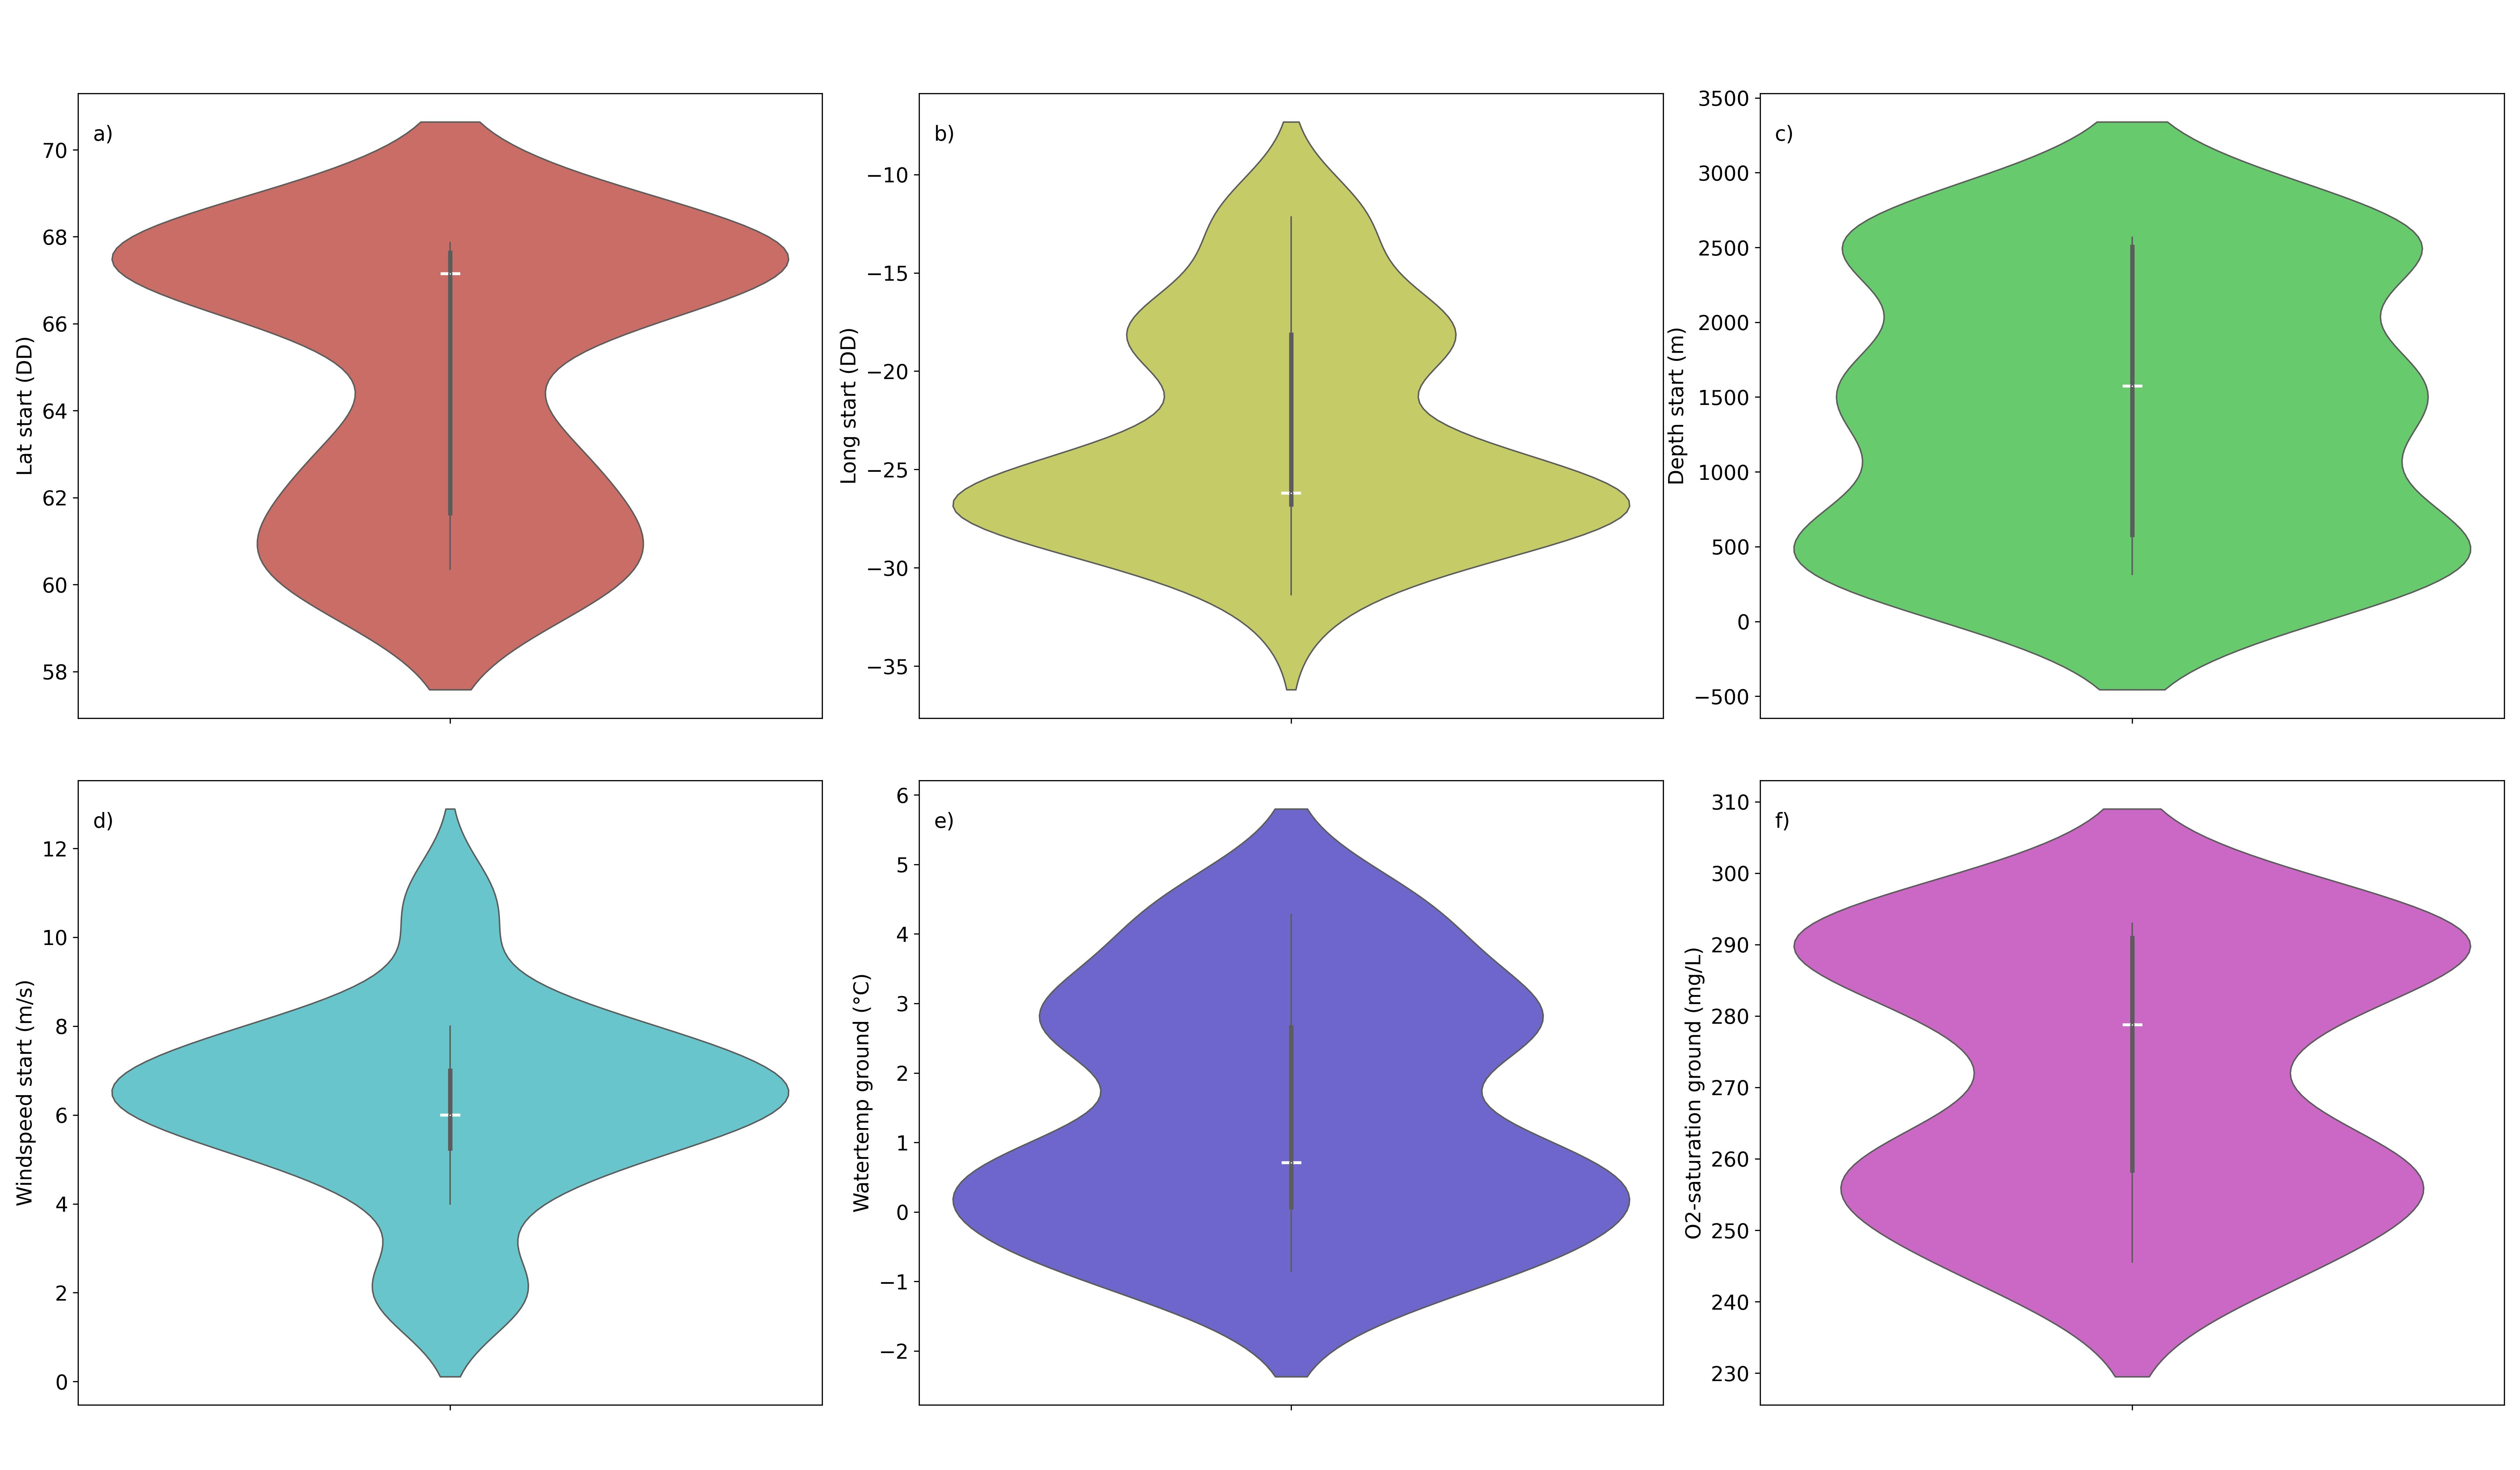
\includegraphics[width=0.7\textwidth]{figure1.jpg}
    \caption{Geographical coordinates at the beginning of the collection of each sample. \label{fig:fig1}}
\end{figure}

\begin{figure}[]
    \centering
    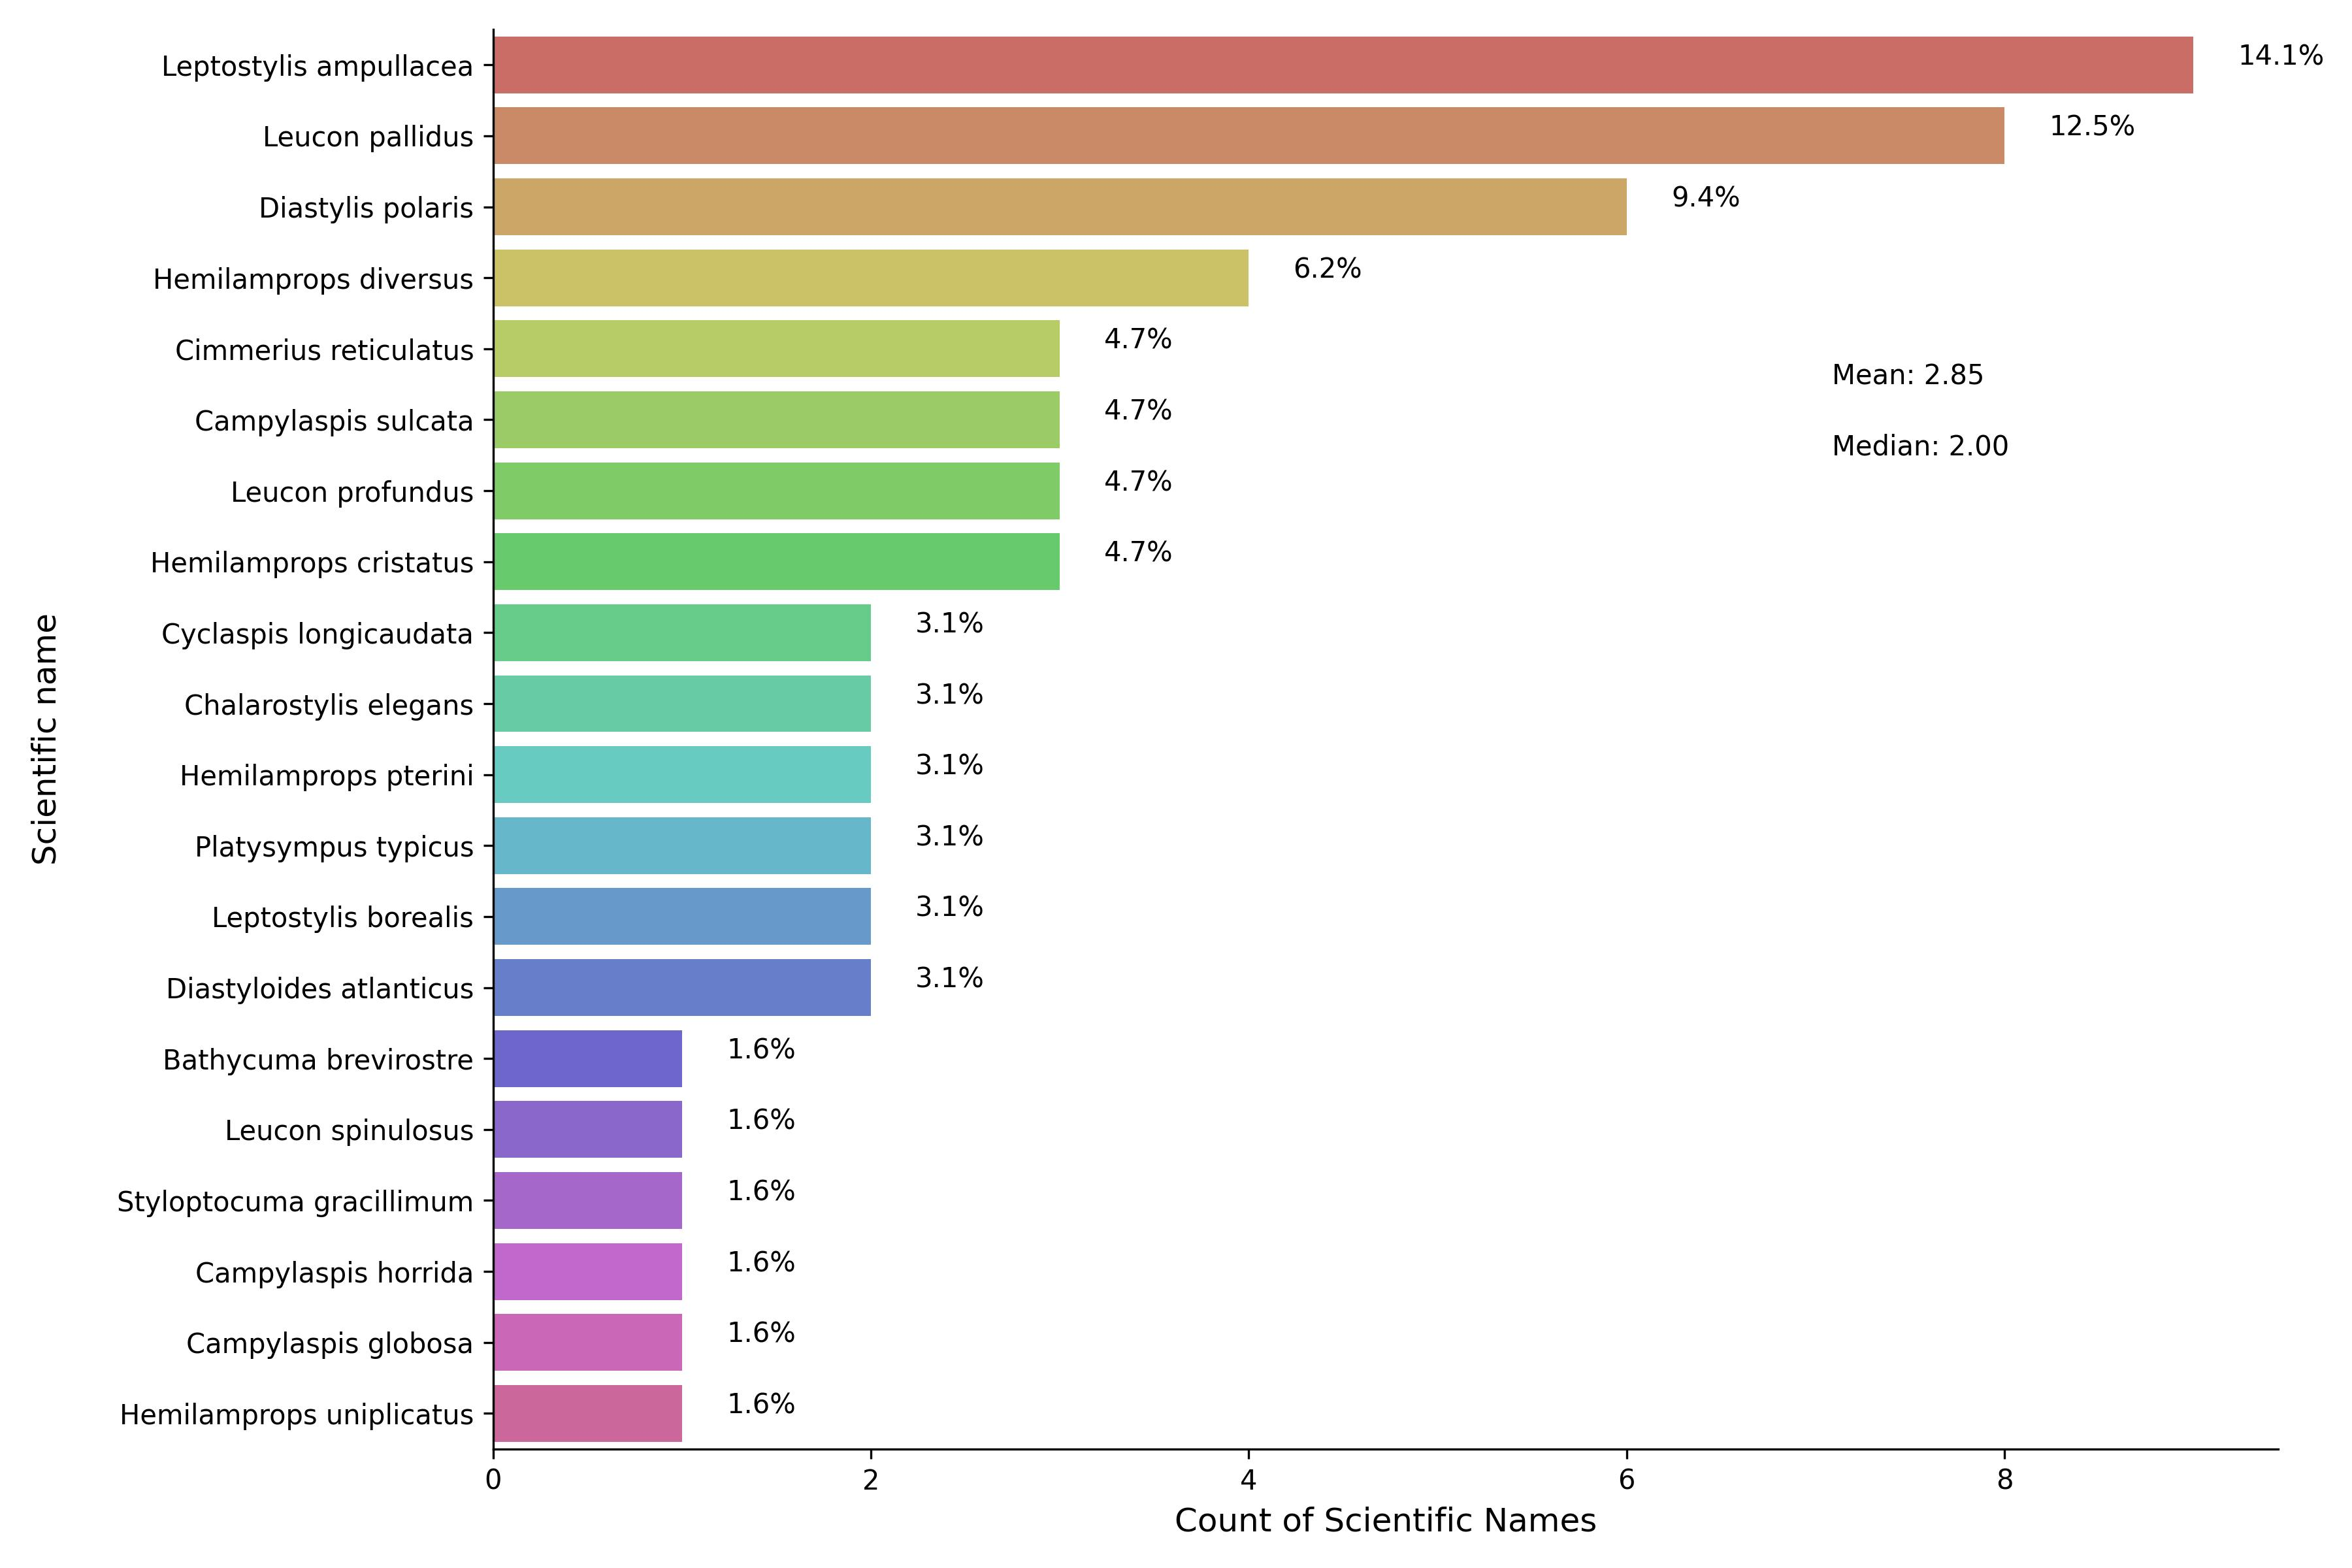
\includegraphics[width=0.7\textwidth]{figure2.jpg}
    \caption{Geographical coordinates at the end of the collection of each sample. \label{fig:fig2}}
\end{figure}

From the IceAGE database, 14 attributes were selected. These consist of the geographical coordinates such as longitude (decimal) and latitude (decimal) taken at the beginning (see Figure \ref{fig:fig1}a and \ref{fig:fig1}b) and at the end of the collection of each sample. The increase in latitude, in particular, has been highlighted by several studies as being linked to the loss of marine biodiversity on a global scale \citep{rex_global-scale_1993, lambshead_latitudinal_2000, gage_diversity_2004}. These geographic data are divided into five sectors across the seas around Iceland: the Denmark Strait (\( n=28 \)), the Iceland Basin (\( n=15 \)), the Irminger Basin (\( n=12 \)), the Norwegian Sea (\( n=4 \)) and the Norwegian Basin (\( n=3 \)). For the environmental attributes in this database, we included the depth (m) at the beginning and end of sampling (see Figure \ref{fig:fig1}c) as well as the temperature (\( \degree C \)) (see Figure \ref{fig:fig1}d) and oxygen concentration (mg/L) (see Figure \ref{fig:fig1}e) of the water depending on the depth at which the specimens were sampled. These properties of water bodies are drivers of deep-sea biodiversity and biogeography with oxygen being a limiting factor for living organisms \citep{keeling_ocean_2010}. In addition to these contributions, the increase in depth \citep{rex_global_2006, costello_marine_2017} as well as the decrease in water temperature at depth \citep{lambshead_latitudinal_2000} are also factors in the loss of marine biodiversity on a global scale. Meteorological parameters such as speed (m/s) (see Figure \ref{fig:fig1}f) and wind direction at the beginning and end of sampling were also included in our data given the contribution of wind to the restructuring of the benthic ecosystem through water transport \citep{saeedi_environmental_2022, waga_recent_2020}. The wind direction at the start of sampling consists of six orientations: South-West (\( n=22 \)), South (\( n=15 \)), North-East (\( n=9 \)), South-South-East (\( n=9 \)), North-West (\( n=5 \)) and East (\( n=2 \)); while the one at the end of the sampling is made up of seven orientations: South (\( n=15 \)), South-West (\( n=15 \)), North-East (\( n=9 \)), West-South-West (\( n=7 \)), South-East (\( n=6 \)), North-North-West (\( n=5 \)), South-South-East (\( n=3 \)) and East (\( n=2 \)). In addition, we have included the sedimentary characteristics of the sampling sites as factors influencing the distribution of Cumacea \citep{uhlir_adding_2021} and which, for the purposes of this study, fall into six categories: mud (\( n=30 \)), sandy mud (\( n=15 \)), sand (\( n=9 \)), forams (\( n=3 \)), muddy sand (\( n=3 \)) and gravel (\( n=2 \)).

\begin{figure}[]
    \centering
    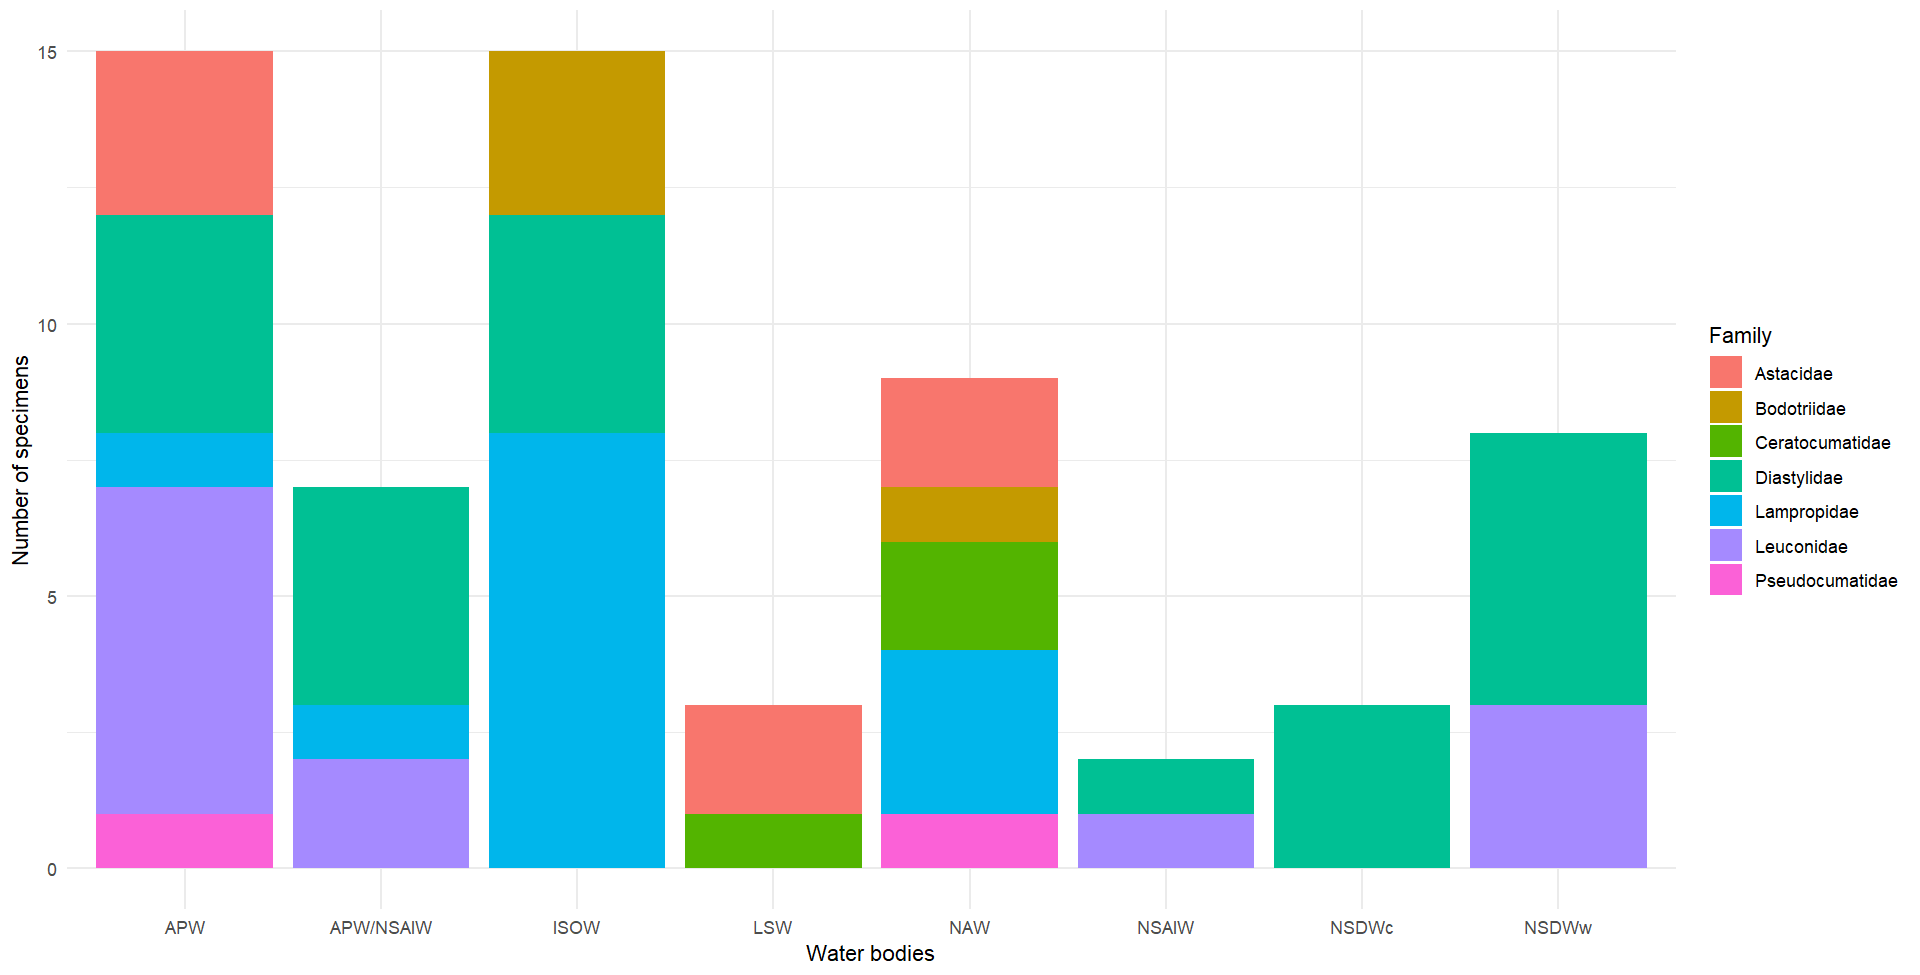
\includegraphics[width=0.7\textwidth]{figure3.png}
    \caption{Depth at the beginning and end of sampling. \label{fig:fig3}}
\end{figure}

\begin{figure}[]
    \centering
    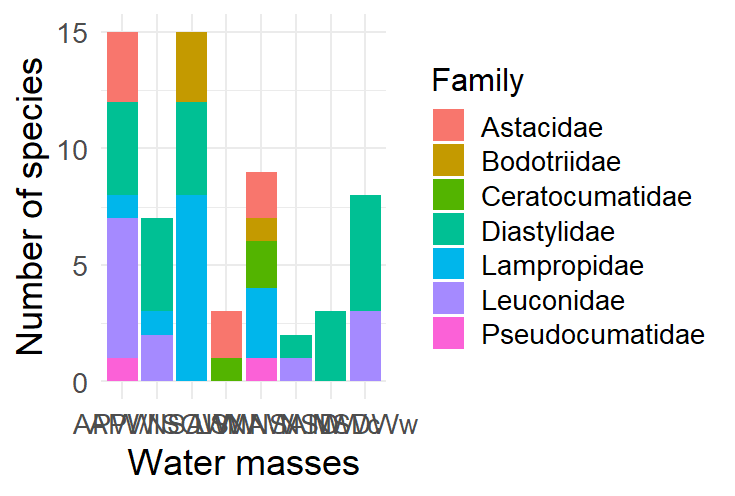
\includegraphics[width=0.7\textwidth]{figure4.png}
    \caption{Temperature (\( \degree C \)) of the water at sampling depth. \label{fig:fig4}}
\end{figure}

\autoref{lst:main}.
\begin{lstlisting}[label=lst:main,language=Python,caption=aPhyloGeo’s main function]
    if __name__ == "__main__":
        print(titleCard + "\n")

        # load params 
        Params.load_from_file()
        sequenceFile = utils.loadSequenceFile(Params.reference_gene_filepath)
        align_sequence = AlignSequences(sequenceFile)

        climatic_data = pd.read_csv(Params.file_name)

        print("\nStarting alignement")
        start_time = time.time()
        alignements = align_sequence.align()

        geneticTrees = utils.geneticPipeline(alignements.msa)
        trees = GeneticTrees(trees_dict=geneticTrees, format="newick")
        end_time = time.time()
        elapsed_time = round(end_time - start_time, 3)
        print(f"Elapsed time: {elapsed_time} seconds")

        climaticTrees = utils.climaticPipeline(climatic_data)
        utils.filterResults(climaticTrees, geneticTrees, climatic_data)

        alignements.save_to_json(f"./results/aligned_{Params.reference_gene_file}.json")
        trees.save_trees_to_json("./results/geneticTrees.json")
\end{lstlisting}

In the BOLD Systems database, taxonomic ranks such as family, genus, and species of the sampled Cumacea were included in our data. These are composed of seven families of Cumacea: Diastylidae (\( n=21 \)), Lampropidae (\( n=13 \)), Leuconidae (\( n=12 \)), Nannastacidae (\( n=7 \)), Bodotriidae (\( n=4 \)), Ceratocumatidae (\( n=3 \)) and Pseudocumatidae (\( n=2 \)). A total of 21 species of Cumacea are found in our sample (see Figure \ref{fig:fig2}).

The habitat and water mass of the sampling points are the only attributes that were taken directly via Table 1 of \cite{uhlir_adding_2021}. Thus, the definitions of water bodies described by \cite{ostmann_marine_2014} were used as a reference for the GIN seas around Iceland: Arctic Polar Water (APW, \( n=15 \)), Iceland Sea Overflow Water (ISOW, \( n=15 \)), North Atlantic Water (NAW, \( n=9 \)), Arctic Polar Water/Norwegian Sea Arctic Intermediate Water (APW/NSAIW, \( n=7 \)), warm Norwegian Sea Deep Water (NSDWw, \( n=8 \)), Labrador Sea Water (LSW, \( n=3 \)), cold Norwegian Sea Deep Water (NSDWc, \( n=3 \)) and Norwegian Sea Arctic Intermediate Water (NSAIW, \( n=2 \)). In terms of habitat, we considered the three categories used in \cite{uhlir_adding_2021}: deep sea (\( n=38 \)), shelf (\( n=15 \)) and slope (\( n=9 \)).

The aligned DNA sequence of the mitochondrial 16S rRNA gene region of each of the samples will also be included in our analyses. Thus, we consider 62 of the 306 aligned DNA sequences that were used for phylogenetic analyses of \cite{uhlir_adding_2021}. Since some of the specimens in our sample have their DNA sequence aligned duplicated, or even quadrupled with a difference of one to two nucleotides, we consider the longest aligned DNA sequence for each of the specimens.

\subsection{aPhyloGeo software}

For our analyses, we use the cross-platform Python software aPhyloGeo designed to analyze phylogenetic trees using climate parameters. Developed by Nadia Tahiri, Georges Marceau and David Beauchemin, the latter offers tools to study the correlations between the genetics of species and their habitats, thus allowing the understanding of the evolution of species under different environmental conditions. The software process takes place in three main steps. 

    The first step is to collect Cumacea DNA sequences of sufficient quality for the requirements of our results \citep{koshkarov_phylogeography_2022}. A total of 62 Cumacea samples were selected to represent 62 sequences of the gene mitochondrial 16S rRNA. Subsequently, we included 6 climatic factors, namely the temperature and O2 concentration of the water as well as the wind speed and direction at the beginning and end of the sample. We also included 9 geographical factors, such as the body of water, the type of habitat and the type of sediment where the samples were collected. The latitude, longitude and depth of sample collection at the beginning and end of sampling were also considered among our geographical parameters.

    In the second step, the trees were generated with climatic, geographical and genetic data. For the geographic parameters, we calculated the dissimilarity between each pair of data from different geographic conditions, which produced a symmetric square matrix. From this matrix, the neighbor junction algorithm was used to design the climate tree. The same approach was applied to climatic and genetic data. Using the 62 sequences of the gene of mitochondrial 16S rRNA, phylogenetic reconstruction is repeated to build gene trees, considering only the data within a range that moves along the alignment. This displacement can vary depending on the steps and window size set by the user (their length is defined by the number of base pairs (pb)) \citep{koshkarov_phylogeography_2022}.

    In the third step, the phylogenetic trees built in each sliding window are compared to climatic and geographic parameters using the Robinson and Foulds (RF) topological distance \citep{robinson_comparison_1981, koshkarov_phylogeography_2022}. The distance was normalized by $2n-6$, where $n$ represents the number of taxa. The approach also considers bootstraping. Thus, the use of the sliding window ensures detailed identification of regions with high genetic mutation rates \citep{koshkarov_phylogeography_2022}.

In short, we want to demonstrate a potential correlation between parts of the genes containing a high rate of mutations according to the geographical distribution of Cumacea samples.

\subsection{Software Update}
The aPhyloGeo software was updated to facilitate these analyses. The updates included improvements to the user interface, enhancements to the data processing algorithms, and the addition of new features for visualizing the results. The updated software is available on GitHub (\url{https://github.com/tahiri-lab/aPhyloGeo}) and PyPi (\href{https://pypi.org/project/aphylogeo/}{PyPi}).

\section{Results}\label{results}

\subsection{Metrics}\label{metrics}

\autoref{lst:LeastSquare}.
\begin{lstlisting}[label=lst:LeastSquare,language=Python,caption=aPhyloGeo’s leastSquare function]
    def leastSquare(tree1, tree2):
        ls = 0.00
        leaves = tree1.get_terminals()

        leavesName = list(map(lambda x: x.name, leaves))
        for i in leavesName:
            leavesName.pop(0)
            for j in leavesName:
                d1 = tree1.distance(tree1.find_any(i), tree1.find_any(j))
                d2 = tree2.distance(tree2.find_any(i), tree2.find_any(j))
                ls += abs(d1 - d2)
        return ls
\end{lstlisting}


\autoref{lst:robinsonFoulds}.
\begin{lstlisting}[label=lst:robinsonFoulds,language=Python,caption=aPhyloGeo’s robinsonFoulds function]
    def robinsonFoulds(tree1, tree2):
        rf = 0
        tree1_newick = ete3.Tree(tree1.format("newick"), format=1)
        tree2_newick = ete3.Tree(tree2.format("newick"), format=1)

        rf, rf_max, common_leaves, x2, x3, x4, x5 = tree1_newick.robinson_foulds(tree2_newick, unrooted_trees=True)
        if len(common_leaves) == 0:
            rf = 0

        return rf, rf / rf_max
\end{lstlisting}

\autoref{lst:euclideanDist}.
\begin{lstlisting}[label=lst:euclideanDist,language=Python,caption=aPhyloGeo’s euclideanDist function]
    def euclideanDist(tree1, tree2):
        ed = 0
        tns = dendropy.TaxonNamespace()
        tree1_tc = dendropy.Tree.get(data=tree1.format("newick"), schema="newick", taxon_namespace=tns)
        tree2_tc = dendropy.Tree.get(data=tree2.format("newick"), schema="newick", taxon_namespace=tns)
        tree1_tc.encode_bipartitions()
        tree2_tc.encode_bipartitions()
        ed = dendropy.calculate.treecompare.euclidean_distance(tree1_tc, tree2_tc)

        return ed
\end{lstlisting}


\begin{figure}[]
    \centering
    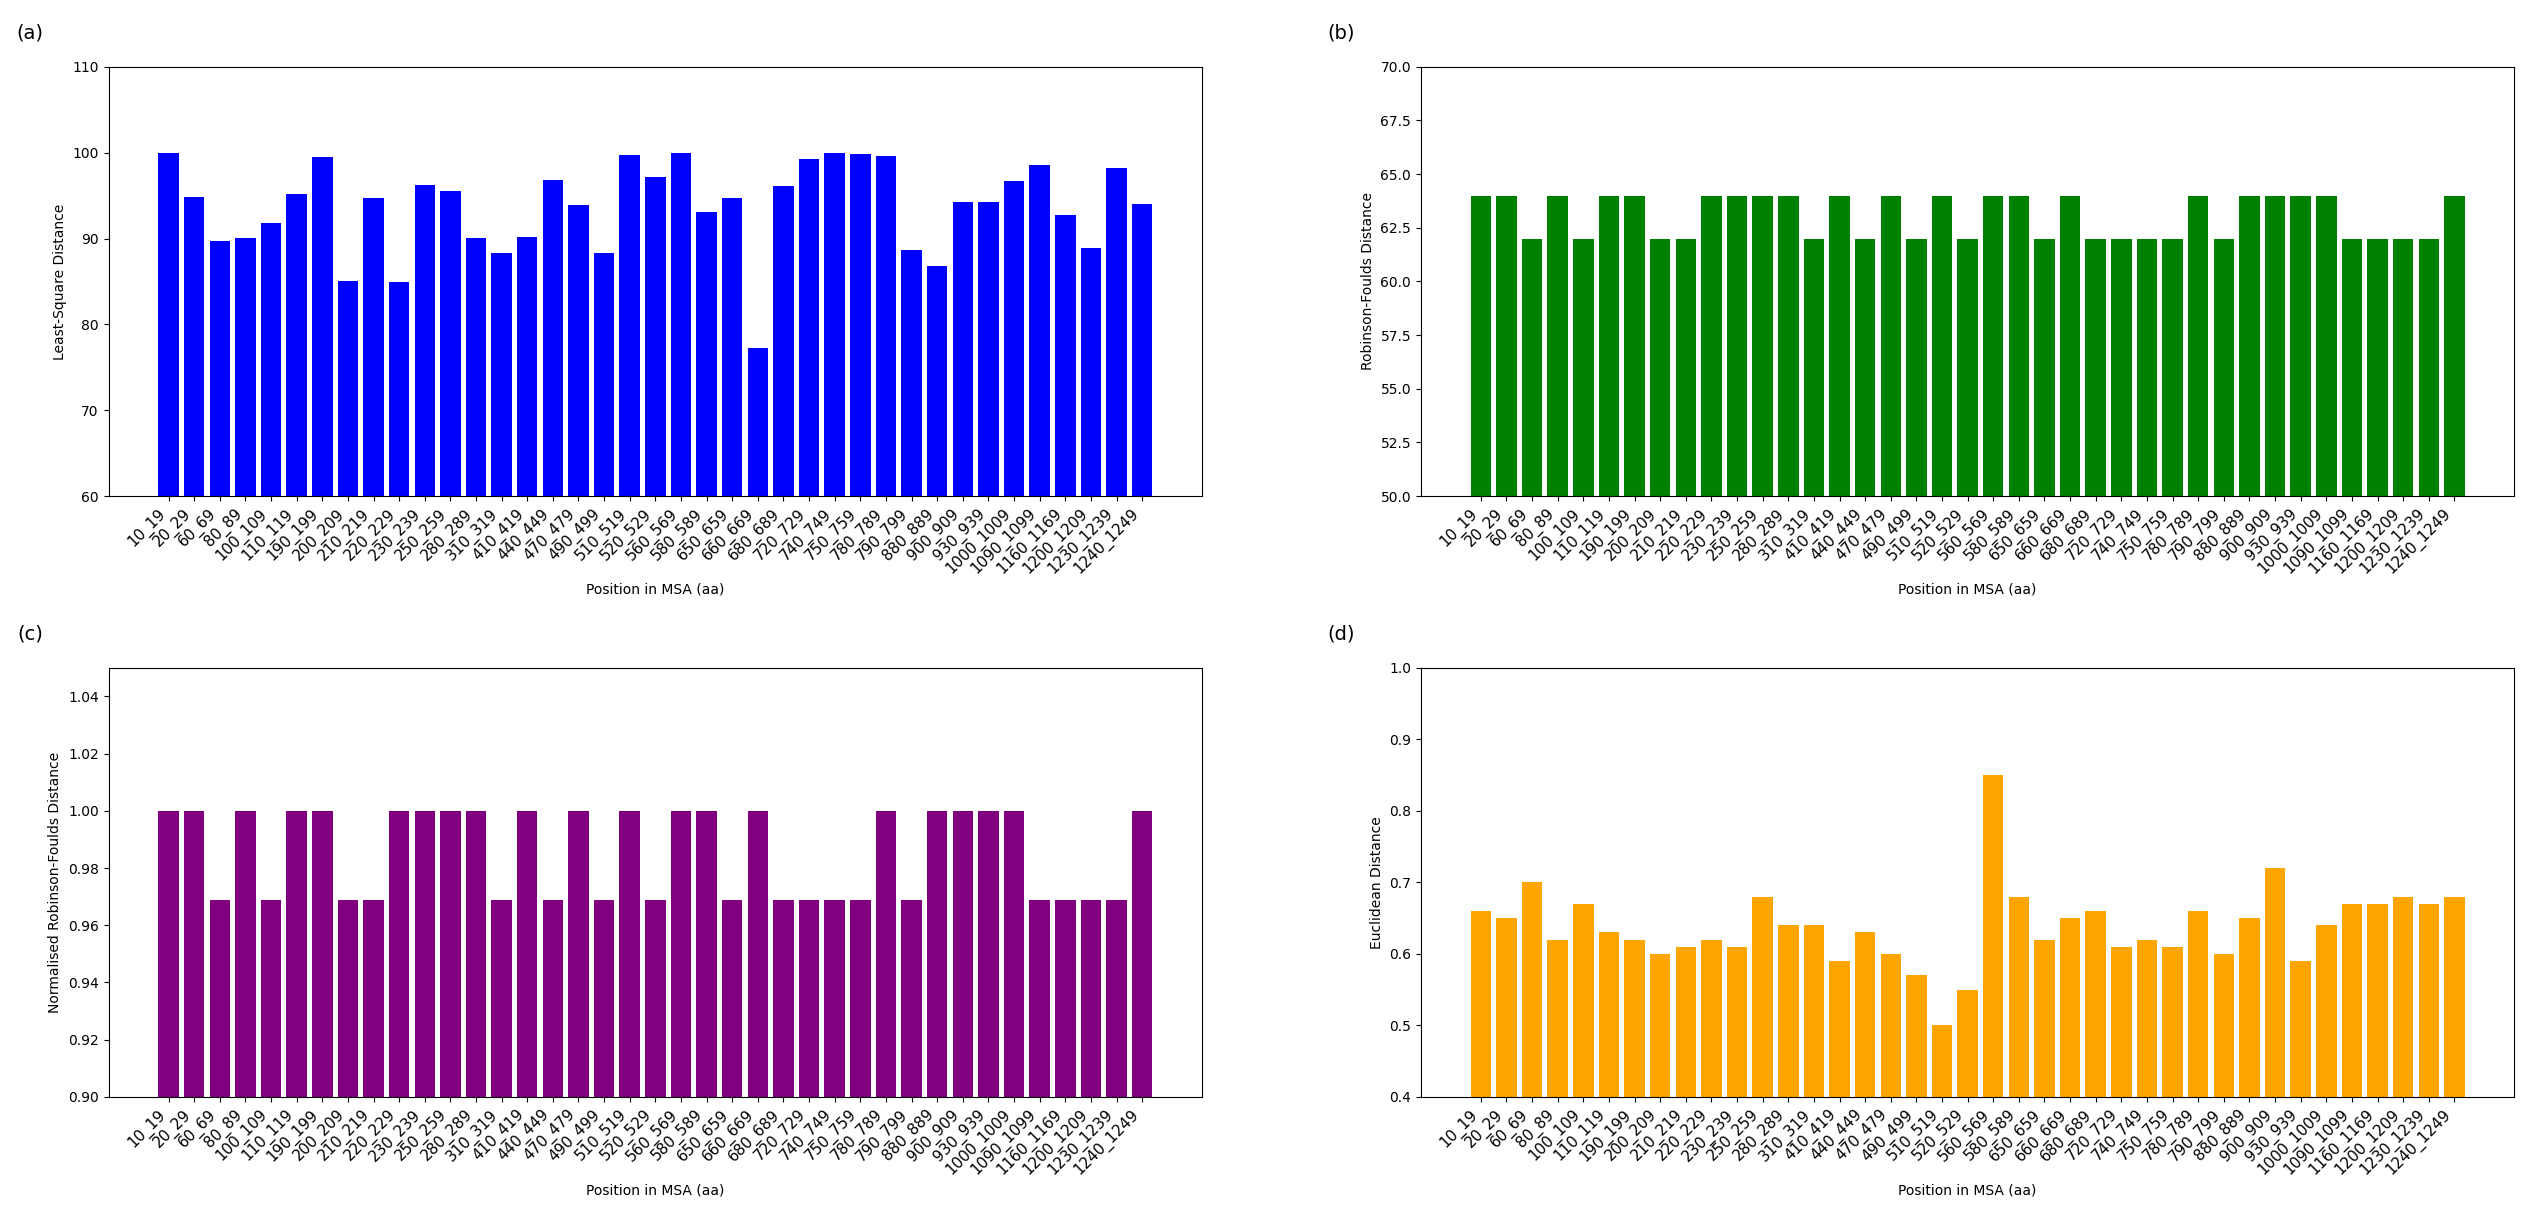
\includegraphics[width=0.7\textwidth]{figure5.png}
    \caption{Variations in the four metrics (Robinson-Foulds distance, generalized Robinson-Foulds, Euclidean distance, and least-square distance) are analyzed to elucidate their correlation with fluctuations in wind speed at the start. \label{fig:fig5}}
\end{figure}

\begin{figure}[]
    \centering
    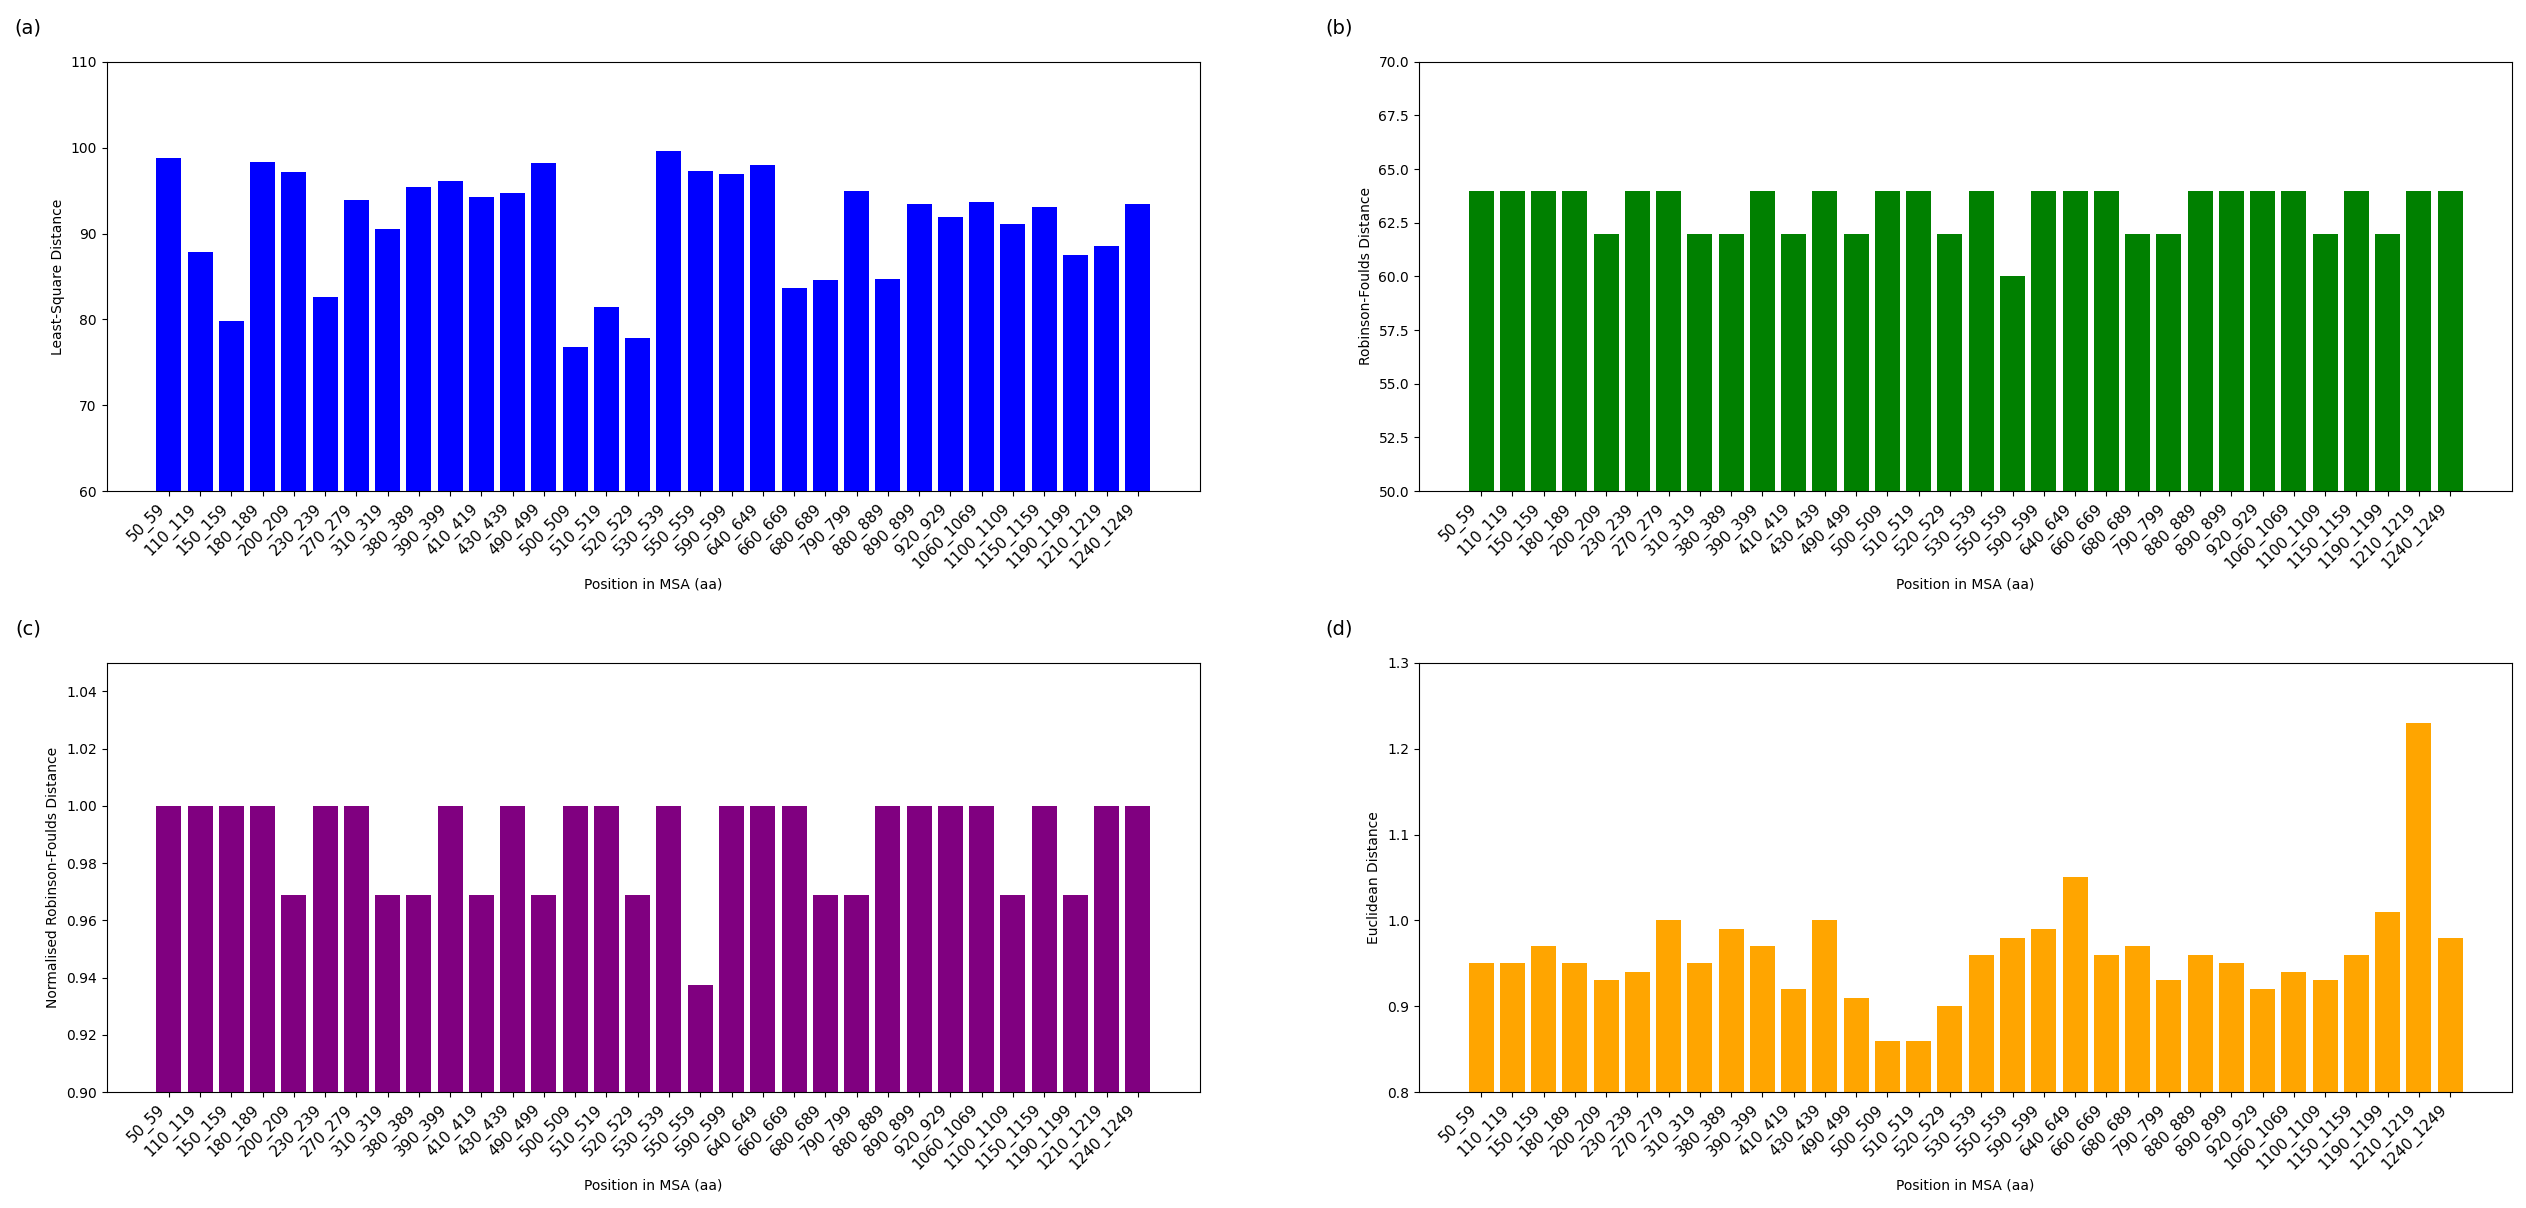
\includegraphics[width=0.7\textwidth]{figure6.png}
    \caption{Variations in the four metrics (Robinson-Foulds distance, generalized Robinson-Foulds, Euclidean distance, and least-square distance) are analyzed to elucidate their correlation with fluctuations in )2 saturation ground. \label{fig:fig6}}
\end{figure}



\section{Conclusion}\label{conclusion}

The objective of this study is to perform an in-depth analysis of the influence of extreme climatic variables and environmental characteristics around Iceland on Cumacea (crustaceans: Peracarida) based on phylogeographic analysis. To date, we have selected relevant attributes for our study based on data from the IceAGE project, BOLD Systems, and the study by \cite{uhlir_adding_2021} and eliminated those that were not relevant to this study as well as those that had low variance (salinity, \( S^2 = 0.02146629 \)) or abundant missing data (>95\%). Thus, the first part consisted mainly of literature review, data collection, data pre-processing, and data analysis.
